\subsection{Covert channel}
We were able to achieve very high accuracy on AMD Zen 3 and Haswell for the case when attacker and victim are in two different processes but have shared memory. For each byte, we had 1000 iterations to detect it. Score in the below figure denotes the number of times out of 1000 that the byte was detected. Score of 999 in almost all cases shows that the attack is very accurate.
\begin{figure}[H]
    \centering
    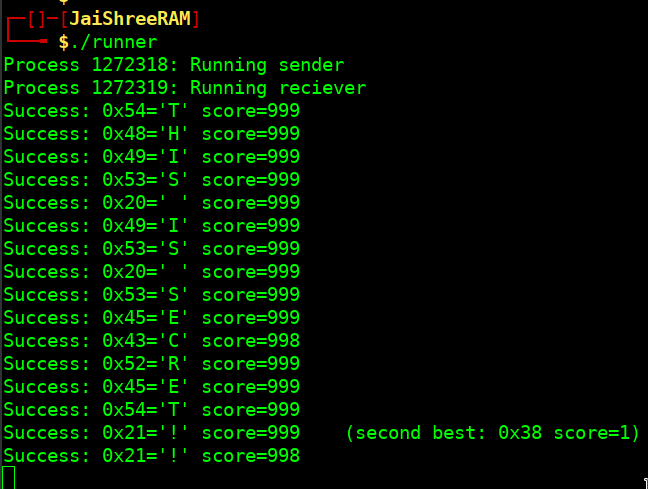
\includegraphics[width=0.4\textwidth]{images/shared-spectre.png}
    \caption{Demonstration of spectre as covert channel}
    \label{covert}
\end{figure}

\subsection{Prime and Probe}
We used the existing code to carry out prime and probe attack on L1D cache. Even in this case attacker and victim reside in the same process. Prime and probe is highly accurate on Haswell architecture but very inaccurate on Alder Lake and Zen 3. We were able to detect the cache lines accessed by the victim with almost 100\% accuracy.
\begin{figure}[H]
    \centering
    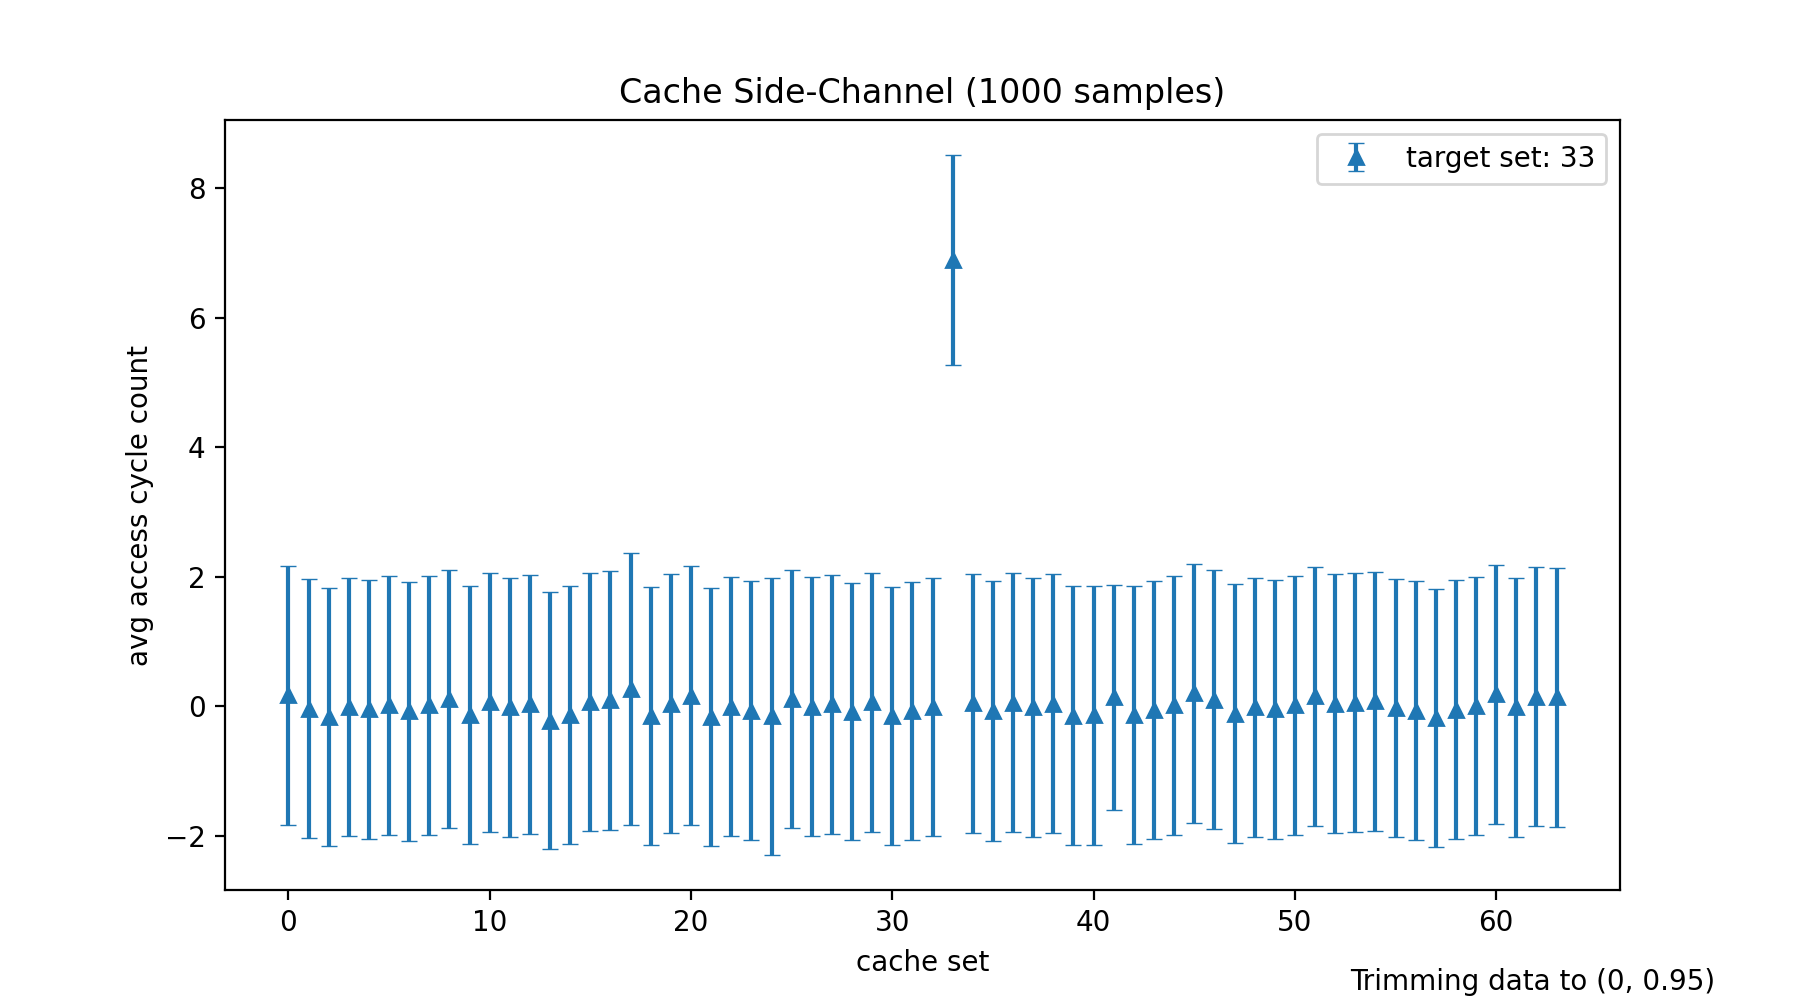
\includegraphics[width=0.5\textwidth]{images/primeprobe.png}
    \caption{Normalized access times of cache sets}
    \label{primeprobe}
\end{figure}
\indent Above figure \ref{primeprobe} shows \textit{normalized} access time of cache sets on Y-axis and set numbering on X-axis. To normalize the times, we first find access times of all cache sets without victim accessing any cache set. Then we subtract these times from the access times of cache sets when victim accesses them. This gives us the normalized access times. We can see the cache set accessed by victim has considerably higher access time than other cache sets. This shows that prime and probe is highly accurate on Haswell architecture.

\subsection{Spectre on unshared memory - single process}
We achieved very high accuracy on Haswell by combining spectre and prime and probe for the case where memory is not shared. Owing to the fact that prime and probe is inaccurate on Alder Lake and Zen 3, we were not able to achieve high accuracy on these architectures. We were able to detect the secret byte with 100\% accuracy on Haswell.
\begin{figure*}[h]
    \centering
    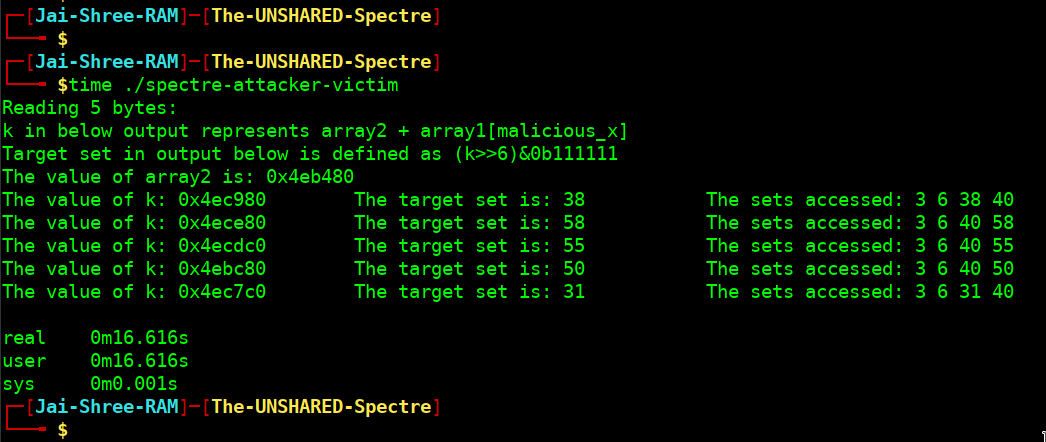
\includegraphics[scale=0.4]{images/unshared-spectre.png}
    \caption{Demonstration of spectre without sharing of memory}
    \label{sidechannel}
\end{figure*}
\indent As we can observe in the Figure \ref{sidechannel}, the secret byte is always detected with 100\% accuracy. But with it, prime and probe also detects few more bytes. But these are constant over every iteration and thus can be filtered out easily. This noise is present owing to the fact that victim also accesses few more memory lines apart from the secret byte, so prime and probe also detects these unwanted lines.

\subsection{Spectre on unshared memory - multiple processes}
We were not able to achieve high accuracy on any of the architectures for this case. Prime and probe is still able to detect the line accessed by victim, but with it many more lines are also being detected. The noise is very high in this case. This is due to the fact that a context switch is needed before the attacker can probe the cache. This context switch brings in many more lines in the cache, thus creating this noise.